 \documentclass[12pt]{article}
\usepackage[T2A]{fontenc}
\usepackage[utf8]{inputenc}       

\usepackage[russian, english]{babel}
\usepackage{amsmath,amsfonts,amsthm,amssymb,amsbsy,amstext,amscd,amsxtra,multicol}
\usepackage{verbatim}
\usepackage{tikz}
\usetikzlibrary{automata,positioning}
\usepackage{multicol}
\usepackage{graphicx}
\usepackage[colorlinks,urlcolor=blue]{hyperref}
\usepackage[stable]{footmisc}
\usepackage{ dsfont }
\usepackage{wrapfig}
\usepackage{xparse}
\usepackage{ifthen}
\usepackage{bm}
\usepackage{color}
 \usepackage{subfigure}
 
\usepackage{algorithm}
\usepackage{algpseudocode}

\usepackage{xcolor}
\usepackage{hyperref}
\definecolor{linkcolor}{HTML}{799B03} % цвет гиперссылок
\definecolor{urlcolor}{HTML}{799B03} % цвет гиперссылок
 
%\hypersetup{pdfstartview=FitH,  linkcolor=linkcolor,urlcolor=urlcolor, colorlinks=true}

\newtheorem{theorem}{Теорема}[section]
\newtheorem{lemma}{Лемма}[section]

\DeclareMathOperator{\sign}{sign}
\DeclareMathOperator{\grad}{grad}
\DeclareMathOperator{\intt}{int}
\DeclareMathOperator{\conv}{conv}
\begin{document}

\tableofcontents
\newpage


\section{Описание метода}

Рассмторим задачу минимизации функции от двух переменных, заданной на квадрате:

$$\min_{(x,y)}\left\{f(x,y)|(x,y) \in Q\right\},$$
где $f$ - это выпуклая функция, $Q$ - квадрат на плоскости. Здесь и далее будем считать, что стороны квадрата соориентированы параллельно осям текущей системы координат. Очевидно, что это не предположение не существенно, поскольку для любого квадрата существует тривиальное афинное преобразование, которое повернет этот квадрат так, чтобы он соответствовал условию

Тогда рассмотрим метод двумерной дихотомии. Его основные этапы следующие:

1. Провести отрезок через центр квадрата параллельно оси Ox.

2. Решить одномерную задачу оптимизации на этом отрезке с некоторой точностью $\delta$

3. Вычислим градиент в полученной точке и отбросим прямоугольник, в который смотрит этот градиент

4. Повторить шаги 2-3 для вертикального отрезка через центр

5. Повторять шаги 1-4, пока не достигнута необходимая точность по функции.

Заметим, что на шаге 3 мы не нуждаемся во всем градиенте, а только в его ортогональной компоненте, т.е. производной по той переменной, которая была фиксировона на текущем отрезке.

Для решения одномерной задачи мы можем использовать любой метод одномерной оптимизации. Однако, в следующих разделах мы покажем, что дифференцируемость функции - существенное условие для сходимости метода, поэтому без ограничения общности мы можем и будем использовать метод дихотомии, использующий производную в центре отрезка, поскольку этот метод гарантирует линейную скорость сходимости и при этом является одноточечным, в отличии, например, от метода золотого сечения или метода дихотомии нулевого порядка.

Утверждается, что для некоторой точности решения вспомогательной задачи $\delta$ данный метод будет сходиться к решению по функции. Это будет обсуждено в следующей секции.

Сейчас обсудим корректность алгоритма. Здесь и далее мы будем использовать следующую нотацию. Пусть мы работаем с некоторым отрезком. Если есть некоторый вектор $\textbf{g}$, то $\textbf{g}_\parallel$ - его проекция на этот отрезок, а $\textbf{g}_\perp$ - его перпендикулярная компонента. Если этот отрезок параллелен одной из осей координат и функция $f(\textbf{x})$ зависит от двух переменных, то $f_\perp'(\textbf{x})$ есть ее производная по компоненте, перпендикулярной этому отрезку, а $f_\parallel'(\textbf{x})$ - по компоненте, параллельной отрезку.

Здесь и далее нам понадобятся стандартные понятия субдифференциала и субградиента, которые можно найти, например, в \cite{Nesterov}.

Нам понадобится следующая лемма.

\begin{lemma}
\label{subgradient}

Если $\textbf{x}_*$ решение одномерной задачи оптимизации:

$$\exists g \in \partial_Q f(\textbf{x}_*) : g_\parallel = 0$$
\end{lemma}
\begin{proof}[Доказательство]
Если $\textbf{x}_*$ есть внутренняя точка, то производная по нефиксированной переменной равна нулю в силу того, что $\textbf{x}_*$ - минимум. Тогда с учетом того, что $\nabla f(\textbf{x}_*)\in\partial f(\textbf{x}_*)$, получаем утвержение из теоремы.

Допустим, что $\textbf{x}_*$ граничная точка. Тогда множество условного субдифференциала на квадрате $Q$ определяется следующим образом:

$$\partial_Q f(\textbf{x}) = \partial f(\textbf{x}) + N\left(\textbf{x}|Q\right),$$
где $N(\textbf{x}|Q) = \left\{\textbf{a}|\langle\textbf{a}, \textbf{y} - \textbf{x}\rangle\leq 0, \forall \textbf{y} \in Q\right\}$. 

Далее предполагаем, что мы решаем задачу оптимизации на горизонтальном сегменте и $\textbf{x}_*$ есть правый конец этого отрезка. Доказательство на три других случая (другой конец горизонтального сегмента и два конца вертикального сегмента). В нашем случае:

$$\partial f(\textbf{x}_*) = \{\nabla f(\textbf{x}_*)\},$$
$$N(\textbf{x}|Q) =\left\{\textbf{a}|\textbf{a}_\perp = 0, \textbf{a}\parallel \geq0\right\}$$

Заметим, что $\left(\nabla f(\textbf{x}_*)\right)_\parallel \leq 0$, потому что, если бы это было не так, то очевидно $\textbf{x}_*$ - не минимум функции $f$ на этом сегменте. Тогда выбрав $\textbf{a}$, такой что $\textbf{a}_\parallel = -\left(\nabla f(\textbf{x}_*)\right)_\parallel$, получаем субградиент из условия:

$$\textbf{g} = \nabla f(\textbf{x}_*) + \textbf{a} : \textbf{g}_\parallel =0$$
\end{proof}

\begin{theorem}
Если функция $f$ выпуклая непрерывно дифференцируемая функция, то для решения  любой одномерной задачи существует некоторая его окрестность, такая что, если выбрать прямоугольник на основе перпендикулярной компоненты градиента в любой точке этой окрестности, выбор будет такой же, как и в случае использования градиента в точке-решении.
\end{theorem}

Данный метод работает не для всех выпуклых функций, даже если решать задачу одномерной оптимизации точно. Пример негладкой выпуклой функции был расмотрен в \cite{Ston_Pas}.

\section{Одномерная задача}
\label{Delta}

В этой секции мы опишем достаточную точность решения вспомогательной задачи на отрезке. Мы будем использовать следующие обозначения:

$$(x_*,y_*) \text{ or }\textbf{x}_*\text{ -- solution of one-dimensional problem} $$
$$\delta = |x-x_*| \text{ -- distance}$$

В работе \cite{Ston_Pas} была доказана следующая теорема:

\begin{theorem}
\label{ConstEst}
Пусть функция $f$ выпуклая и удовлетворяет условие Липшица с константой $M$, а ее градиент - с константой $L$.
Тогда если каждая одномерная задача решена со следующей точностью по аргументу
\begin{equation}
\delta \leq \frac{\epsilon}{2La(\sqrt{2}+\sqrt{5})(1-\frac{\epsilon}{Ma\sqrt{2}})}
\end{equation}
то метод двумерной дихотомии сходится к решению с точностью $\epsilon$ по функции.
\end{theorem}

Данная стратегия всегда требует решать задачу с точностью порядка $\epsilon$. А также данный метод может не гарантировать сходимости по аргументу. Такой пример также был рассмотрен в работе \cite{Ston_Pas}. Далее мы будем называть эту стратегию \textbf{ConstEst}(Constant Estimate).

Теперь разработаем стратегию, которая гарантирует сходимость по аргументу. Заметим, что прямоугольник выбирается правильно, если знак производной в решении вспомогательной задачи совпадает со знаком производной в ее приближении:

\begin{equation}\label{MCH}
f'_\perp(\textbf{x}_*)f'_\perp(\textbf{x}_*+\delta) > 0
\end{equation}

Здесь и далее мы будем использовать следующую простую лемму:

\begin{lemma}
\label{trick_lemma}
$\forall a,b\in\mathbb{R}\backslash\{0\}, |a-b|\leq |b| \Rightarrow \sign a = \sign b$
\end{lemma}
\begin{proof}[Доказательство]
Если $b>0$ и $a\leq b$, тогда условие из леммы эквивалентно следующему:
$$b-a\leq b\Rightarrow a\geq 0.$$
Если $b>0$ и $a \geq b$, тогда $a\geq 0$.

Случай отрицательного $b$ доказывается аналогично.
\end{proof}

\begin{theorem}
\label{CurGrad}
Пусть функция $f$ выпуклая с липшецевым градиентом с константой $L$. Точка $\textbf{x}_*$ решение одномерной задачи оптимизации, $\textbf{x}$ - ее приближение.

Тогда если приближение удовлетворяет следующему условию:

$$\delta \leq \frac{|f_\perp'(\textbf{x})|}{L},$$
то прямоугольник, выбранный на основе градиента в этой точке, содержит решение исходной задачи на квадрате. 
\end{theorem}
\begin{proof}[Доказательство]

Из леммы \ref{trick_lemma} следует, что для того чтобы совпали знаки, достаточно потребовать

$$\left|f'_\perp(\textbf{x}_*) - f'_\perp(\textbf{x})\right| \leq |f'_\perp(\textbf{x})|$$

Используя липшецевость градиента получаем утверждение теоремы.
\end{proof}

Описанная в теореме оценка крайне не эффективна, если модуль перпендикулярной компоненты стремительно убывает при приближении к точке-решению, поэтому сформулируем альтернативное условие остановки:

\begin{theorem}
\label{small}
Пусть $f$ есть $M$-липшецева выпуклая с $L$-липшецевым градиентов. Точка $\textbf{x}_*$ есть решение одномерной задачи оптимизации, $\textbf{x}$ - ее приближение, $\delta = \|\textbf{x}_*-\textbf{x}\|$ - верхняя оценка расстояния между ними.

Тогда для достижения точности $\epsilon$ в точке $\textbf{x}$ следующего условия достаточно:
$$\delta \leq \frac{\epsilon-LR|f_\perp'(x)|}{L+MR}, $$
где $R=a\sqrt{2}$ это размер диагонали квадрата.
\end{theorem}

\begin{proof}[Доказательство]

Из леммы \ref{subgradient} мы имеем:

$$g \in \partial f(\textbf{x}_*): g_\parallel = 0.$$

Тогда по определению субградиента:

$$f(\textbf{x}^*) - f(\textbf{x}_*) \geq (g, \textbf{x}^* - \textbf{x}_*)$$

Используем неравенство Коши-Буняковского-Шварца:
$$f(\textbf{x}_*) - f(\textbf{x}^*) \leq -(g, \textbf{x}^* - \textbf{x}_* )\leq$$
$$\leq \|g\| \|\textbf{x}^* - \textbf{x}_*\|\leq \|g\|a\sqrt{2}$$

С другой стороны, из липшецевости функции мы имеем:
$$f(\textbf{x})-f(\textbf{x}_*)\leq M\delta$$

$$f(\textbf{x})-f(\textbf{x}^*) \leq M\delta +\|g\|a\sqrt{2} = M\delta + |f_\perp'(\textbf{x}_*)|R$$

Из липшецевости градиента:
$$f(\textbf{x})-f(\textbf{x}^*) \leq M\delta + \left(|f_\perp'(\textbf{x})|+L\delta\right)R$$

Тогда для достижения точности $\epsilon$ по функции в точке $\textbf{x}$ для исходной задачи достаточно следующего условия:

$$M\delta +\|g\|a\sqrt{2} = M\delta + \left(|f_\perp'(\textbf{x})|+L\delta\right)R \leq \epsilon$$

$$\delta \leq \frac{\epsilon - |f_\perp'(\textbf{x})|}{M+LR}$$
\end{proof}


Определим нашу адаптивную стратегию. Мы решаем задачу одномерной оптимизации, пока не выполнено условие на точность по аргументу:

\begin{equation}
\label{Adaptive}
\delta \leq \max\left\{
	\frac{|f_\perp'(\textbf{x})|}{L}, 
	\frac{\epsilon - |f_\perp'(\textbf{x})|}{M+LR}
	\right\}.
\end{equation}

Причем, если выполнено условие из теоремы \ref{small}, мы останавливаем весь метод. Эту стратегию мы назвали \textbf{CurGrad}(Current Gradient).


\section{Сходимость}

В этой сецкии будут приведены оценки для количества итераций глобального метода для достижения точности по функции. В данном разделе под итерацией подразумевается одна итерация метода двумерной дихотомии, в результате которой квадрат уменьшается вдвое.

\begin{theorem}
Если функция $f$ выпуклая и $Ь$-липшецева, тогда для достижения $\epsilon$ по функции следующего количества итераций достаточно:
\begin{equation}\label{NI1}N = \left\lceil\log_2\frac{\sqrt{2}Ma}{\epsilon}\right\rceil\end{equation}
где $a$ размер исходного квадрата $Q$.
\end{theorem}

Доказательство для стратегии \textbf{ConstEst} было проведено в работе \cite{StonPas}. Для стратегии \textbf{CurGrad} данная оценка есть очевидное следствие липшецевости функции и сходимости по аргументу.

Однако мы можем улучшить нашу оценку, если учтем сходимость по аргументу.
\begin{theorem}
Пусть $f$ - выпуклая функция.

Если

1. Функция $f$ имеет $L$-липшецев градиент

2. $\exists \textbf{x}^*\in Q: \nabla f(\textbf{x}^*) = \textbf{0}$

3. Стратегия для решения одномерной задачи обеспечивает сходимость по аргументу

тогда для достижения точности $\epsilon$ по функции следующего количества итераций достаточно:
\begin{equation}\label{NI3}N = \left\lceil\frac{1}{2}\log_2\frac{La^2}{4\epsilon}\right\rceil,
\end{equation}
где $a$ - размер исходного квадрата $Q$.
\end{theorem}

\begin{proof}[Доказательство]
Для всех выпуклых дифференцируемых функций следующее неравенство верно (доказательство можно найти в \cite{Nesterov}):
$$f(\textbf{x}) - f(\textbf{x}^*) - (f'(\textbf{x}^*), \textbf{x} - \textbf{x}^*) \leq \frac{L}{2}\|\textbf{x}-\textbf{x}^*\|^2$$

По условию теоремы существует такая точка $\textbf{x}^*$, что $f'(\textbf{x}^*) = 0$. Заметим, что эта точка является решением задачи. Тогда наше неравенство примет вид:

$$f(\textbf{x}) - f(\textbf{x}^*)\leq \frac{L}{2}\|\textbf{x}-\textbf{x}^*\|^2$$

После $N$ итераций имеем следующую оценку:

$$f(\textbf{x}) - f(\textbf{x}^*)\leq L\left(\frac{a}{2^N}\right)^2,$$
что доказывает оценку из теоремы.
\end{proof}


\section{Двойственные задачи}
\label{details}

Данный метод предполагает особый интерес в приложении решения двойственных задач для задач с двумя ограничениями. А именно, для решения задач вида:

\begin{gather}
\phi(\lambda_1, \lambda_2) \rightarrow \min_{\lambda\geq 0},\\
\text{where } \phi = -\min_\textbf{x}\left(f(\textbf{x}) + \lambda_1 g_1(\textbf{x}) + \lambda_2 g_2(\textbf{x})\right)
\end{gather}
$$\textbf{x}(\lambda) = \arg\min_\textbf{x}\Phi(\textbf{x}, \lambda)$$


В данной секции мы обсудим как свести это к нашей задаче, как вычислить липшецевы константы и каким образом вычислять $\textbf{x}(\lambda)$.

Для начала приведем задачу к задаче минимизации на квадрате. Согласно \cite{task} (see ex. 4.1), мы имеем следующую локализацию на решение:

\begin{gather}
\label{restr:dual}
\|{\lambda}\|_1 \leq a = \frac{1}{\gamma}\left(f(\overline{\textbf{x}}) -\min\limits_{\textbf{x}}f(\textbf{x})\right),\\
\text{где $\overline{\textbf{x}}:g_i(\overline{\textbf{x}})<0,\gamma = \min\limits_i[-g_i(\overline{\textbf{x}})]$}
\end{gather}
Согласно этому утверждению, мы можем локализовать $\lambda^*$ в квадрате $Q = [0, a]^2$. В таком случае мы свели нашу задачу оптимизации к следующему виду:
\begin{gather}
\label{dual}
\phi(\lambda_1, \lambda_2) \rightarrow \min_{\lambda \in Q}
\end{gather}

Градиент функции $\phi$ мы будем считать согласно хорошо известной теорема Демьянова-Данскина-Рубинова, см. \cite{DDR-theorem}.

\begin{theorem}
Пусть $\phi(\lambda)=\min\limits_{x\in X}\Phi(x,\lambda)$ для всех $\lambda\geq0$, где $\Phi$ это гладкая выпуклая функция по $\lambda$. Тогда
$$\nabla \phi(\lambda) = F'_\lambda\left(x(\lambda),\lambda\right)$$
\end{theorem}

Условия теоремы выполнено в нашем случае и мы получаем:
\begin{equation}
\phi'_{\lambda_k}(\lambda) = g_k\left(\textbf{x}(\lambda)\right)
\end{equation}

Кроме этого, мы нуждаемся в константе Липшица для градиента. В работе \cite{Stonykin} сформулирована и доказана следующая теорема:
\begin{theorem}
Пусть $f(x)$ есть $\mu_f$-сильно выпуклая функция, функция $g(x)$ удовлетворяет условию Липшица с константой $M_g$. Тогда функция $\phi(\lambda) = \min_\textbf{x}\left(f(\textbf{x}+\lambda_1g_1(\textbf{x}) + \lambda_2g_2(\textbf{x})\right)$, определенная в \ref{phi}, где $x(\lambda) = \arg\min\limits_x(f(x)+\lambda g(x))$, имеет липшецев градиент с константой $L_{\phi'} = \frac{M_g^2}{\mu_f}$
\end{theorem}

В случае размерности 2 по $\lambda$ доказательство повторяется практически в точности. В таком случае, $g(\textbf{x})$ есть вектор-функция.

Основная сложность решения седловых задач есть то, что вычисление $\textbf{x}(\lambda)$ точно в большинстве случаев невозможно. Следовательно, мы не имеем доступа к точному значению градиента. Это приводит к следующим проблемам:

1. Шаг дихотомии на отрезке

2. Проверка стоп-условия из стратегии \textbf{CurGrad}

3. Выбор прямоугольника

Заметим, что нас в каждой из задач интересуют следующие величины:

1. Проекция градиента на отрезок, т.е. $g_\parallel(\textbf{x}(\lambda))$.

2. Значение разниц $\delta-\frac{|g_\perp(\textbf{x}(\lambda))|}{L}$, где $L$ это липшецева константа для градиента $\phi$.

3. Перпендикулярная компонента, т.е. $g_\perp(\textbf{x}(\lambda))$.

Согласно \cite{Ston_Pas}, мы можем вычислять производные неточно, для того чтобы выбрать прямоугольник с $\epsilon$-решением. Так, если $\delta$ - это точность по аргументу текущего приближения одномерной задачи, и $\Delta$ - точность вычисления градиента в точке по величине градиента, то следующего условия достаточно для нужного выбора прямоугольника:

$$2\Delta + L\delta \leq \frac{\epsilon}{2a(\sqrt{2}+\sqrt{5})},$$
где $L$ - это липшецева константа градиента для двойственной задачи. Мы можем увидеть, что задача выбора сегмента с решением одномерной задачи является одномерным вариантом той же проблемы. Это приводит нас к следующей теореме.

\begin{theorem}
\label{StonPas_Dual}
Если одномерная задача решается со следующей точностью $delta =  \frac{\epsilon}{4La(\sqrt{2}+\sqrt{5})}$ по аргументо, тогда, для того чтобы выбрать прямоугольник с $\epsilon$-решением, достаточно вычислять $\textbf{x}(\lambda)$ в текущей точке со следующей точностью:

\begin{equation}
\|\textbf{x} - \textbf{x}(\lambda)\| \leq \frac{1}{M_g}\frac{\epsilon}{8a(\sqrt{2}+\sqrt{5})}
\end{equation}

Для того, чтобы выбрать сегмент с решением одномерной задачи, достаточно вычислять $\textbf{x}(\lambda)$ в центре текущего сегмента со следующей точностью:
\begin{equation}
\|\textbf{x} - \textbf{x}(\lambda)\| \leq \frac{1}{M_g}\frac{\epsilon}{4a(\sqrt{2}+\sqrt{5})}
\end{equation}
\end{theorem}

С другой стороны, для каждого случая интересен только знак соответствующих выражений. Для этого мы будем применять  лемму \ref{trick_lemma}. Согласно этой лемме, мы имеем следующие достаточные условия для остановки вычисления $\textbf{x}(\lambda)$ для выше обозначенных случаев:

1. $|g_\parallel(\textbf{x})-g_\parallel(\textbf{x})|\leq |g_\parallel(\textbf{x})|$

2. $\frac{1}{L}\Big||g_\perp(\textbf{x})|-|g_\perp(\textbf{x}(\lambda))|\Big|\leq \Big|\delta-\frac{|g_\perp(\textbf{x})|}{L}\Big|$

3. $|g_\perp(\textbf{x})-g_\perp(\textbf{x}(\lambda))|\leq |g_\perp(\textbf{x})|$

Тогда сформулируем утверждения:

\begin{theorem}\label{x_lambda}
Пусть $g_k$ есть $L_{g_k}$-липшецевы функции. Тогда следующие утверждения верны.

1. Для того, чтобы сделать шаг дихотомии корректно, т.е. сохраняя сходимость по аргументу, достаточно вычислять $\textbf{x}(\lambda)$, пока не выполнено следующее условие
$$L_{g_\parallel}\|\textbf{x}-\textbf{x}(\lambda)\|\leq |g_\parallel(\textbf{x})|.$$

2. Для того, чтобы проверить условие останова из стратегии, достаточно вычислять $\textbf{x}(\lambda)$, пока не выполнено следующее условие
$$\frac{L_{g_\perp}}{L}\|\textbf{x}-\textbf{x}(\lambda)\|\leq\Big|\delta-\frac{|g_\perp(\textbf{x})|}{L}\Big|,$$
где $\delta$ это расстояние между текущей $\lambda$ и решением одномерной задачи $\lambda_*$.

3. Для того, чтобы выбрать прямоугольник согласно стратегии, достаточно вычислять $\textbf{x}(\lambda)$, пока не выполнено следующее условие
$$L_{g_\perp}\|\textbf{x}-\textbf{x}(\lambda)\|\leq |g_\perp(\textbf{x})|.$$
\end{theorem}

Выше предложенный способ проверки условий требует сходимости метода по аргументу. Следующая теорема позволит использовать в точке $\epsilon$-субградиент, который, как известно, совпадает с градиентом функции в точке по внутренней переменной в точке $x_\epsilon$ - точке-решении внутренней задачи с точностью $\epsilon$.

\begin{theorem}

Пусть задано выпуклое множество $Q$ и на этом множестве определена выпуклая дифференцируемая функция $f$, при этом ее градиент удовлетворяет условию Липшица с константой $L$. Тогда любой ее $\epsilon$-субградиент будет отличаться от ее градиента не более чем на $\sqrt{\frac{L\epsilon}{2}}$, т.е.

$$\|\partial_\epsilon f(\textbf{x}) - \nabla f(\textbf{x})\| \leq \sqrt{\frac{L\epsilon}{2}},$$

если расстояние от $\textbf{x}$ до границы $Q$ меньше, чем $\sqrt{\frac{\epsilon}{2L}}$.
\end{theorem}

Сделаем два замечания.

Во-первых, вычисление $\textbf{x}(\lambda)$ не зависит от требуемой точности $\epsilon$ для исходной задачи в том смысле, что если мы вычислили $\textbf{x}(\lambda)$ в некоторой точке для некоторого $\epsilon$, то для всех меньших $\epsilon$ мы также будем вычислять это значение, причем за такое же время.

Во-вторых, стратегии, обозначенные в выше сформулированной теореме, не гарантируют сходимости. Например, рассмотрим условие $L_{g_\parallel}\|\textbf{x}-\textbf{x}(\lambda)\|\leq |g_\parallel(\textbf{x})|.$ Если $g_\parallel(\textbf{x}(\lambda))=0$ и левая часть будет убывать медленнее правой, то это условие не будет выполнено. Для того, чтобы избежать этого, предлагается использовать комбинированную стратегию из выше написанных теорем, т.е. высчитывать $\textbf{x}(\lambda)$, пока не будет выполнено одно из условий. Хотелось бы отметить, что в наших экспериментах, описанных ниже, не наблюдалось таких случаев, что условие из теоремы не достижимо.

\section{Сложность}

Оценим сложность решения одномерной проблемы.

Для стратегии \textbf{ConstEst} мы имеем, что одномерная задача требует в точности следующее количество итераций одномерного метода:

$$\log_2\frac{2La(\sqrt{2}+\sqrt{5})(1-\frac{\epsilon}{Ma\sqrt{2}})}{\epsilon} = O\left(\log \frac{1}{\epsilon}\right)$$

Теперь рассмотрим стратегию \textbf{CurGrad}. Пусть модуль перпендикулярной компоненты в точке-решении $|f'_\perp(\lambda_*)|$ равен $\tilde{\epsilon}$, точка $\lambda$ - это приближение $\lambda_*$, $\delta=\|\lambda-\lambda_*\|$.

Если мы используем метод дихотомии и $N$ - это количество итераций дихотомии, из $L$-липшецевости градиета мы имеем следующую оценку:

$$\tilde{\epsilon}-La2^{-N} \leq |f_\perp'(\lambda)|\leq \tilde{\epsilon}+La2^{-N}.$$

Согласно этоц оценке, чтобы достичь необходимой точности в первом выражении в максимуме из оценки \ref{Adaptive} следующего количества итераций достаточно:

$$a2^{-N} \leq \frac{\tilde{\epsilon}-La2^{-N}}{L}$$
Для второго выражения в максимуме имеем условие:
$$a2^{-N} \leq \frac{\epsilon - \tilde{\epsilon} - La2^{-N}}{M+LR}\leq \frac{\epsilon - \tilde{\epsilon}}{M+LR} - La2^{-N}$$

Тогда согласно этим оценкам, чтобы достичь выполнения условия \ref{Adaptive}, нам достаточно следующее количество итераций:
$$1+\log_2\min\left\{\frac{La}{\tilde{\epsilon}},\frac{(M+LR)a}{\epsilon-\tilde{\epsilon}}\right\}$$

Худший случай набдюдается при следующих значениях
$$\tilde{\epsilon} = \frac{L}{оценкуM+L(R+1)}\epsilon.$$
В этом случае нам достаточно следующее количество итераций:
$$1+\log_2\frac{(M+L(R+1))a}{\epsilon} = O\left(\log\frac{1}{\epsilon}\right)$$

Из этой оценки следует, что адаптивная стратегия в худшем случае работает так же, как и стратегия \textbf{ConstGrad}, т.е. \textbf{CurGrad} не хуже \textbf{ConstGrad}. 

Таким образом для одномерной задачи требуется $O\left(\log \frac{1}{\epsilon}\right)$ итераций.

\begin{theorem}
Для того, чтобы достичь точности $\epsilon$ по функции, двумерная дихотомия требует следующее количество вычислений значения функции $f$ и ее производных первого порядка:
$$O\left(\log^2\frac{1}{\epsilon}\right)$$
\end{theorem} 
\begin{proof}[Доказательство]
Мы доказали, что для решения одномерной задачи требуется следующее количество итераций:
$$\log_2\frac{Ca}{\epsilon},$$
где $C$ - константа, определеяемая стратегией и зависящая от констант Липшица для функции и градиента.

На $N$-ой итерации двумерной дихотомии требуется решить две одномерные задачи на сегменте размера $a_N=a2^{-N}$. Из оценок на количество итераций двумерной дихотомии получаем, что всего мы сделаем $N_{\max}=\log_2\frac{1}{\epsilon}+O(1)$ итераций. Тогда можем оценить количество обращений к оракулу первого порядка:

$$\sum_{k=0}^{N_{\max}}\log_2\frac{Ca2^{-k}}{\epsilon} = $$
$$= \sum_{k=0}^{N_{\max}}\log_2\frac{Ca}{\epsilon} - \sum_{k=0}^{N_{\max}}k=$$
$$= N_{\max}\log_2\frac{Ca}{\epsilon} - \frac{1}{2}N_{\max}^2 + O\left(\log\frac{1}{\epsilon}\right)=$$

$$= \frac{1}{2}\log_2^2\frac{1}{\epsilon} +O\left(\log\frac{1}{\epsilon}\right)=$$
$$=O\left(\log^2\frac{1}{\epsilon}\right)$$
\end{proof}

В случае решения седловых задач мы имеем сложность, верхняя оценка которой также зависит от $\epsilon$. Пусть мы рассматриваем задачу
\begin{gather}
\phi(\lambda_1, \lambda_2) \rightarrow \min_{\lambda\geq 0},\\
\text{where } \phi = -\min_\textbf{x}\left(f(\textbf{x}) + \lambda_1 g_1(\textbf{x}) + \lambda_2 g_2(\textbf{x})\right)
\end{gather}
Если функция $f$ сильно выпуклая, то следующего количества обращений к оракулу первого порядка для $f$ и $g_k$ достаточно, чтобы достичь точности $\epsilon$ по функции в двойственной задаче:
$$O(\log^3\frac{1}{\epsilon})$$

В данном разделе приведены оценки для худшего случая, на практике метод сходится сильно лучше.

\section{Другие неточные методы}
\label{Inexact}

В этой секции мы обсудим другие неточные методы, которые не нуждаются в точном значении градиента и функции в точке, чтобы сходиться  к решению с некоторой заранее заданной точностью.

Во-первых, это Primal Gradient Method (PGM) с $(\delta, L,\mu)$ оракулом. В \cite{PGM} было доказано, что это метод сходится к решению с точностью $\delta$ со слеующей скоростью:
$$\min_k f(\textbf{x}_k) - f(\textbf{x}^*) \leq \frac{LR^2}{2}\exp\left(-k\frac{\mu}{L}\right) + \delta,$$
где $R = \|\textbf{x}_0-\textbf{x}^*\|$. Более того, в \cite{PGM} доказано, что для функции вида
$$f(\textbf{x}) = \min\limits_\textbf{u} \left(\Psi(\textbf{x},\textbf{u}) + \textbf{u}^\top A\textbf{x}\right)$$
существует следующий $(\delta, L,\mu)$-оракул:
$$f_{\delta, L,\mu}(\textbf{x}) = \Psi(\textbf{x}, \textbf{u}_\textbf{x}) - \xi$$
$$g_{\delta, L,\mu}(\textbf{x}) = A\textbf{u}_\textbf{x}$$
с параметрами $\delta = 3\xi$, $L = \frac{2\lambda_{\max}(A^\top A)}{\mu(G)}$, $\mu = \frac{\lambda_{\min}(A^\top A)}{2L(G)}$, если $\textbf{u}_\textbf{x}$ это приближение решения $\textbf{u}^*$ в текущей точке $\textbf{x}$ с точностью $\xi$ по функции.

Вторым методом будет Fast Gradient Method с $(\delta, L,\mu)$ оракулом. Этот метод также сходится к решению с точностю $\delta$ со следующей скоростью:
$$\min_k f(\textbf{x}_k) - f(\textbf{x}^*) \leq \min\left(\frac{4LR^2}{k^2}, LR^2\exp\left(-\frac{k}{2}\sqrt{\frac{\mu}{L}}\right)\right) + C_k\delta,$$
где $C_k = \min\left(\frac{k}{3}+\frac{12}{5}, 1+\sqrt\frac{L}{\mu}\right)$. Описание этого метода также можно найти в \cite{PGM}.


Третий метод - это неточный метод эллипсоидов. Этот метод использует $\epsilon$-субградиент вместо обычного и сходится к $\epsilon$-решению:
$$\min_k f(\textbf{x}_k) - f(\textbf{x}^*)\leq \max_{\textbf{x}\in Q}|f(\textbf{x})|\exp\left(-\frac{k}{8}\right)+\delta$$
Это доказано в \cite{Ellipsoids}. Более того, в книге \cite{Polyak} доказано, что для функции
$$f(\textbf{x}) = \min\limits_\textbf{u}\Psi(\textbf{x},\textbf{u})$$
мы можем найти $\epsilon$-субградиент:
$$\Psi(\textbf{x},\textbf{u}_{\textbf{x},\epsilon})\in\partial_\epsilon f(\textbf{x}),$$
есди $\textbf{u}_{\textbf{x},\epsilon}$ это такая точка, что $\Psi(\textbf{x},\textbf{u}_{\textbf{x},\epsilon}) - \min\limits_\textbf{u}\Psi(\textbf{x},\textbf{u})\leq\epsilon$.

\section{Эксперименты}
\label{Comparison}


В этом разделе мы приведем сравнение неточных методов (см. \ref{Inexact}) с предложенным в этой статье на примере двойственной задачи по времени работы\footnote{Вы можете найти весь код в репозитории~\cite{my_git}}. Весь код был сделана на Anaconda 5.3.1 Python 3.6 (см.~\cite{conda}).

\begin{figure}[ht!]  
\vspace{-4ex} \centering \subfigure[]{
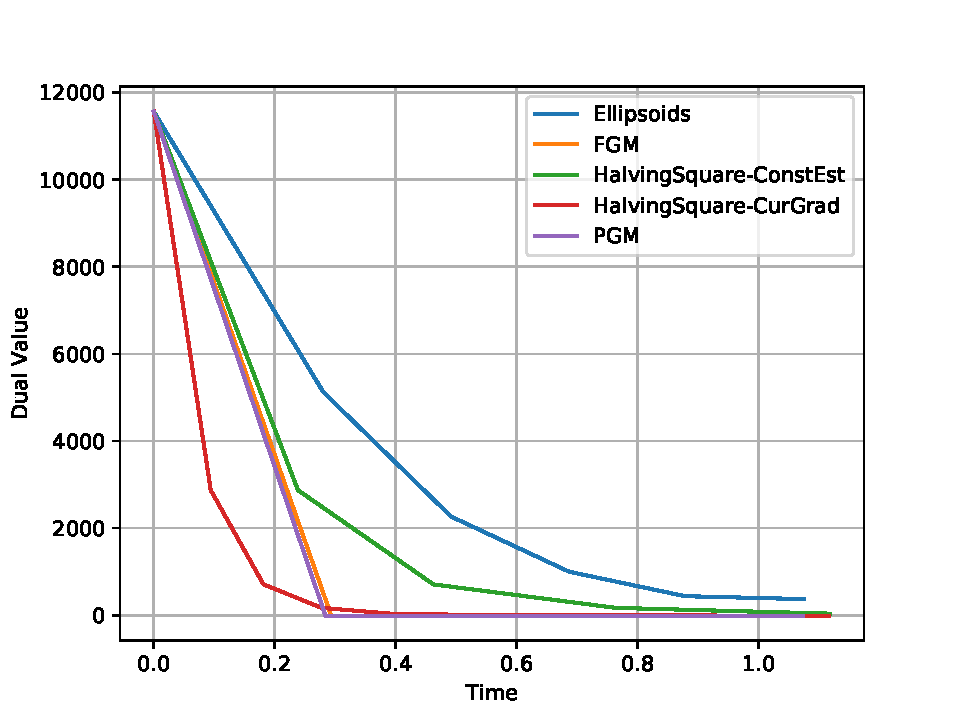
\includegraphics[width=0.25\linewidth]{../Tests/Images/1000_1e-03.pdf} \label{100_3} }  
\hspace{2ex}
\subfigure[]{
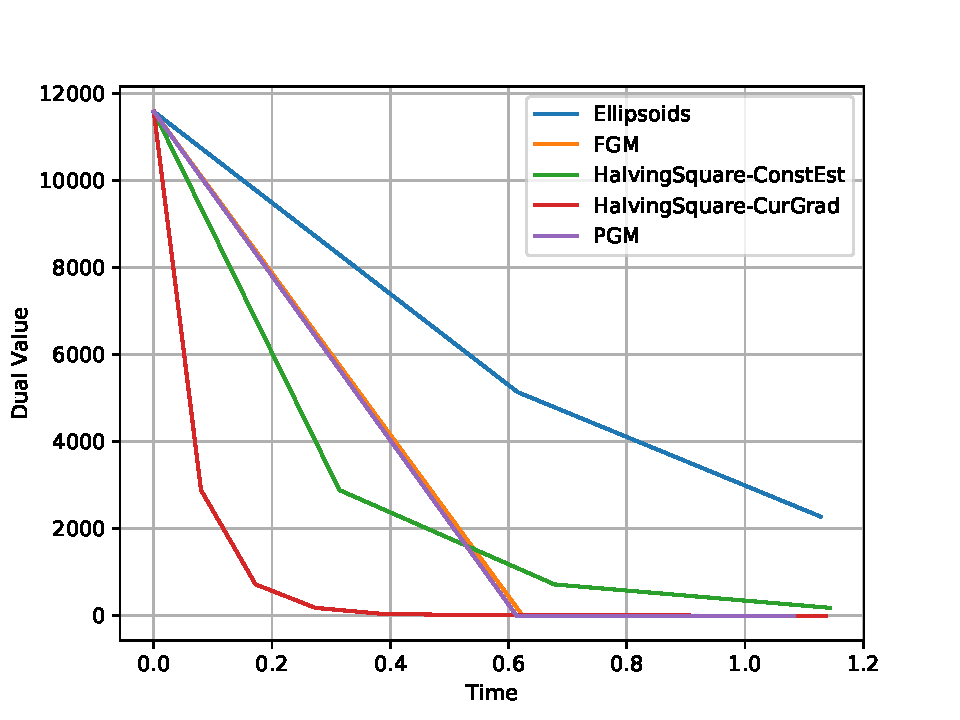
\includegraphics[width=0.25\linewidth]{../Tests/Images/1000_1e-10.pdf} \label{100_10} }
\vspace{2ex}
\subfigure[]{
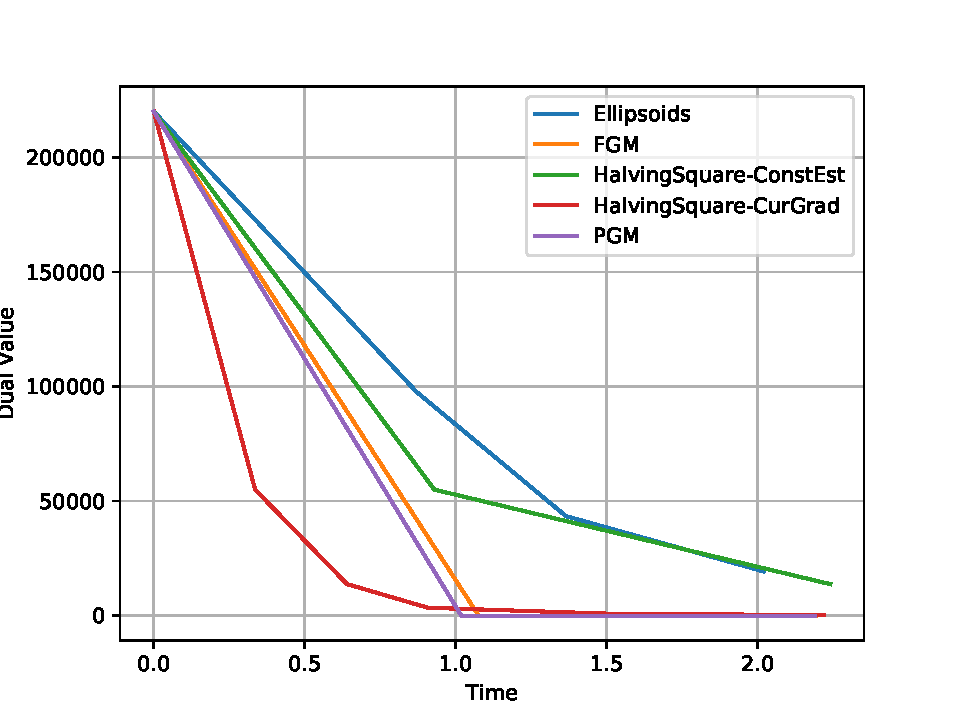
\includegraphics[width=0.25\linewidth]{../Tests/Images/10000_1e-03.pdf} \label{1000_3} }  
\hspace{2ex}
\subfigure[]{
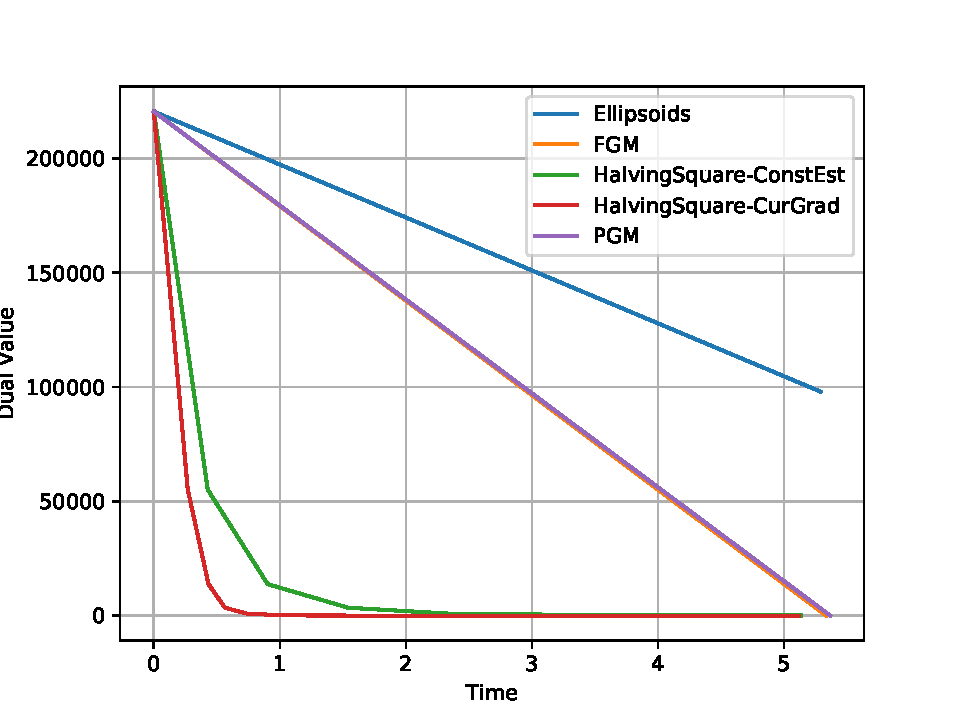
\includegraphics[width=0.25\linewidth]{../Tests/Images/10000_1e-10.pdf} \label{1000_10} }
\vspace{2ex}
\subfigure[]{
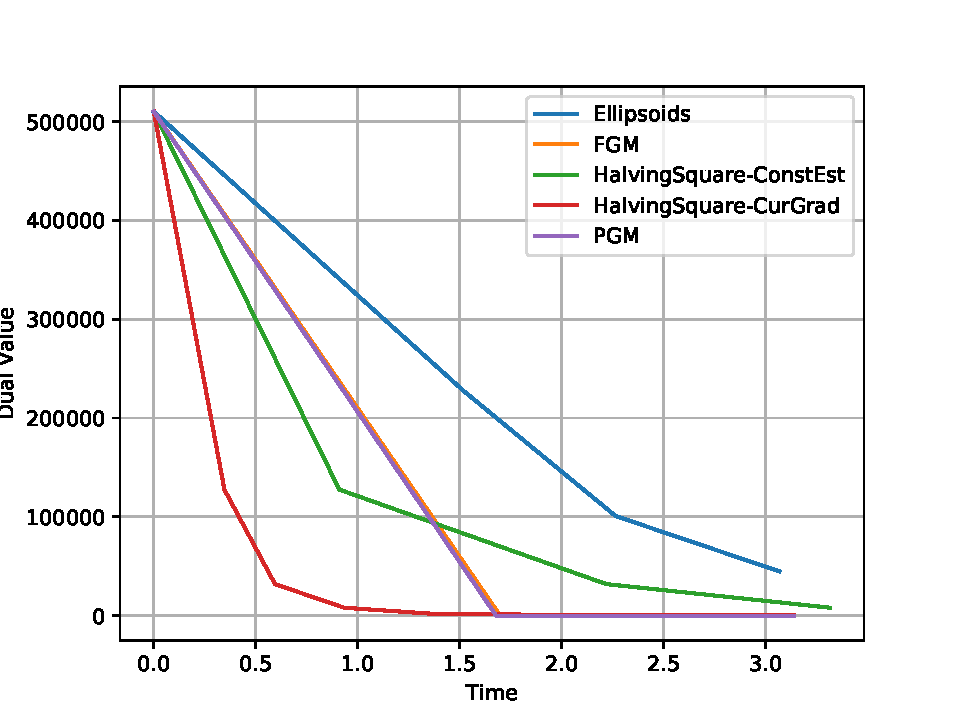
\includegraphics[width=0.25\linewidth]{../Tests/Images/20000_1e-03.pdf} \label{10000_3} }  
\hspace{2ex}
\subfigure[]{
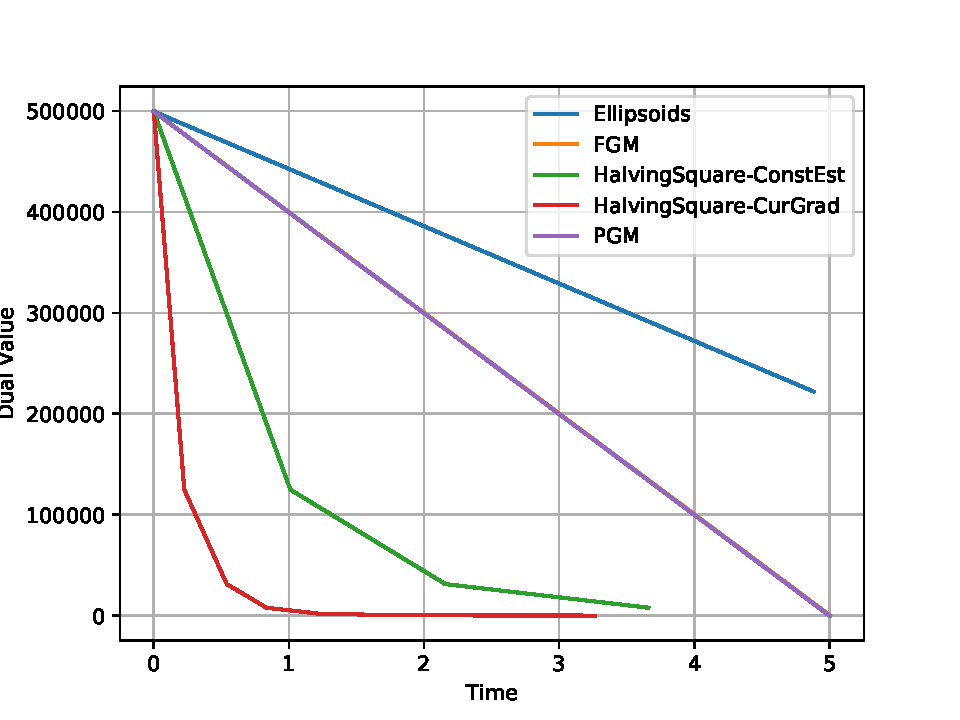
\includegraphics[width=0.25\linewidth]{../Tests/Images/20000_1e-10.pdf} \label{10000_10} }
\hspace{2ex}
\caption{Сравнение различных неточных методов на двойственных задачах с различными размерностями прямой задачи $N$ и различными требуемыми точностями $\epsilon$: \subref{100_3} $N=1000,\epsilon=10^{-3}$; \subref{100_10} $N=1000,\epsilon=10^{-10}$; \subref{1000_3} $N=10000,\epsilon=10^{-3}$; \subref{1000_10} $N=10000,\epsilon=10^{-10}$; \subref{10000_3} $N=20000,\epsilon=10^{-3}$; \subref{10000_10} $N=20000,\epsilon=10^{-10}$. } \label{fig:image}
\end{figure}

Для нахождения $\textbf{x}(\lambda)$ мы будем использовать градиентный спуск. Есть следующие результаты для теоретической скорости сходимости:

Если $f$ есть $\mu$-сильно выпуклая функция с $L$-липшецевым градиентом, то градиентынй спуск с шагом $\alpha_k = \frac{1}{L+\mu}$ сходится со следующей скоростью
$$\|f(\textbf{x}_k)-f(\textbf{x}^*)\|\leq \left(\frac{M-1}{M+1}\right)^kL\|\textbf{x}_0-\textbf{x}^*\|,$$
$$\|\textbf{x}_k-\textbf{x}^*\|\leq \left(\frac{M-1}{M+1}\right)^k\|\textbf{x}_0-\textbf{x}^*\|,$$
где $M =\frac{L}{\mu}$. Доказательство этого факта можно найти в \cite{Polyak}.

Для всех неточных методов высчитываем $\textbf{x}(\lambda)$, пока теоретическая скорость сходимости градиентного спуска не гарантирует достаточного условия для того, чтобы наш неточный метод сошелся к решению с точностью $\epsilon$ по функции. Так для PGM, FGM и неточного метода эллипсоидов мы вычисляем $\textbf{x}(\lambda)$ с точностью $\frac{\epsilon}{2}$ по функции. Для нашего метода для обоих стратегий условия останова были обсуждены в секции \ref{dual}.

Рассмотрим следующую задачу:
\begin{gather}
\label{prime}
f(\textbf{x}) = \ln \left(1+\sum_{k=1}^ne^{\alpha x_k}\right) + \beta\|\textbf{x}\|_2^2\rightarrow \min\limits_{\textbf{x}\in \mathbb{R}^N}\\
g_k(\textbf{x}) = \langle \textbf{b}_k, \textbf{x}\rangle+c_k\leq0, k = \overline{1,m}\\
\end{gather}

Это задача минимизации LogSumExp-функции с $l_2$-регуляризацией. Параметр регуляризации $\beta$ равен параметру сильной выпуклости для этой задачи, и в наших экспериментах мы брали его равным $0.01$. Число $N$ - это размерность прямой задачи и определяется  в разных экспериментах по разному. Параметр $\alpha$ взят равным $1.0$. Парметры $c_k$ для простоты также взяты равными $1.0$. Векторы $\{\textbf{b}_k\}_{k=1}^m$ для каждого эксперимента генерируются случайно из равномерного распределения на $[0, 1.0]^N$. Параметр $m$ равен размерности двойственной задачи и равен двум.

Минимизируемая функция $f$ есть $L$-липшицева функция с $M$-липшецевым градиентом, где $L=1$ and $M=\alpha$. В таком случае имеем:
$$L_f = \alpha+2\beta R, M_f = \alpha^2 + 2\beta,$$
$$\mu_f = 2\beta,$$
где $R=\|\textbf{x}_0-\textbf{x}^*\|$ это расстояние от решения до начального приближения. Функции $g_k$ есть $L_k$-липшецевы с параметрами $L_k=\|b_k\|$. 

Используем следующую нотацию:
\begin{equation}
\label{phi}
\phi(\lambda_1, \lambda_2) = -\min\limits_{\textbf{x}\in \mathbb{R}^N}\left(f(\textbf{x}) +\lambda_1 g_1(\textbf{x}) +\lambda_2g_2(\textbf{x})\right)
\end{equation}

В такой нотации, двойственная задача \ref{prime} выглядит следующим образом
\begin{gather}
\phi(\lambda_1, \lambda_2) \rightarrow \min\limits_{\lambda_1, \lambda_2}\\
\text{s.t}\, \lambda_1, \lambda_2 \geq 0
\end{gather}
 
Очевидно, что $\min\limits_{\textbf{x}}f(\textbf{x}) \geq 0$. Тогда, согласно \ref{restr:dual},  мы имеем следующую локализацию решения:
$$|\lambda_k| \leq \lambda_{\text{max}}=\frac{f(\overline{\textbf{x}})}{\gamma}, k=1,2$$

И получаем следующую задачу:
$$\phi(\lambda_1, \lambda_2) \rightarrow \min_{0\leq\lambda_k\leq\lambda_{max}}$$

На рис.~\ref{fig:image} мы видим следующие результаты. Во-первых, двумерная дихотомия показывает сравнительно хороший результат, когда задача нахождения $\textbf{x}(\lambda)$ "сложная", т.е. размерность прямой задачи или требуемая точность являются высокими. Во-вторых, наш метод со стратегией \textbf{CurGrad} показывает наилучший результат для таких сложных задач.

\newpage
\begin{thebibliography}{3}
\bibitem{task}
Gasnikov A.  Universal gradient descent // MIPT --- 2018, 240 p.
\bibitem{Ston_Pas}
Pasechnyk D.A., Stonyakin F.S.  One method for minimization a convex Lipchitz continuous function of two variables on a fixed square // arXiv.org e-Print archive. 2018. – URL: \href{https://arxiv.org/pdf/1812.10300.pdf}{https://arxiv.org/pdf/1812.10300.pdf}
\bibitem{Nesterov}
Nesterov U.E.  Methods of convex optimization // M.MCNMO --- 2010, 262 p.
\bibitem{conda}
Anaconda[site]. At available: \href{https://www.anaconda.com}{https://www.anaconda.com}
\bibitem{DDR-theorem}
Danskin, J.M.: The theory of Max-Min, with applications. J. SIAM Appl. Math.14(4) (1966)
\bibitem{Stonykin}
Fedor S. Stonyakin, Mohammad S. Alkousa, Alexander A. Titov,and Victoria V. Piskunova1 On Some Methods for Strongly Convex Optimization Problems with One Functional Constraint // ...
\bibitem{PGM}
Olivier Devolder Exactness, Inexactness and Stochasticityin First-Order Methods for Large-ScaleConvex Optimization // UCL --- 2013,
\bibitem{Ellipsoids}
Need Reference To Book with Inexact Ellipsoids
\bibitem{Polyak}
B.T. Polyak. The Introduction to Optimization // Moscow, Science - 1983
\bibitem{my_git}
Repository with code: \href{https://github.com/ASEDOS999/Optimization-Halving-The-Square}{https://github.com/ASEDOS999/Optimization-Halving-The-Square}
\end{thebibliography}
\end{document}
